220. а)\begin{figure}[ht!]
\center{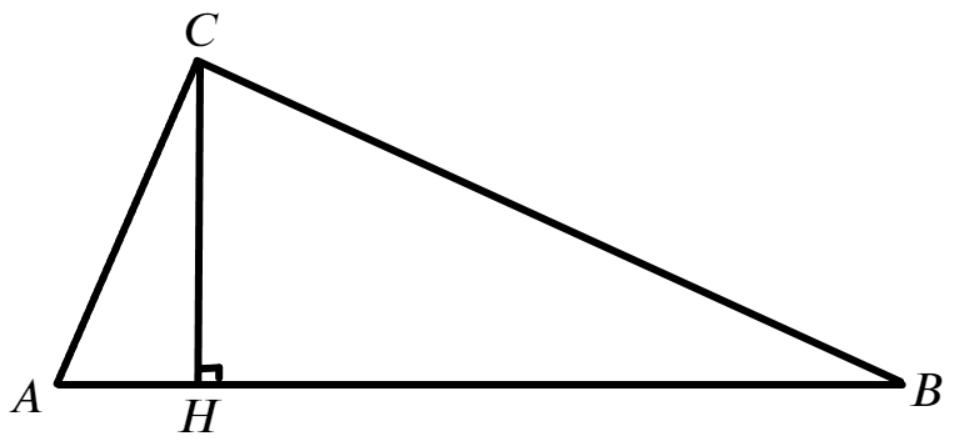
\includegraphics[scale=0.35]{g8-220b.png}}
\end{figure}\\
Если $CH^2=AH\cdot HB,$ то $\cfrac{CH}{AH}=\cfrac{HB}{CH}$ и треугольники $CHB$ и $AHC$ подобны по двум сторонам и углу между ними $(\angle AHC=\angle BHC=90^\circ).$ Тогда $\angle B=\angle ACH=90^\circ-\angle A,$ поэтому $\angle C=180^\circ-\angle A-\angle B=90^\circ,$ ч.т.д.\\
б) \begin{figure}[ht!]
\center{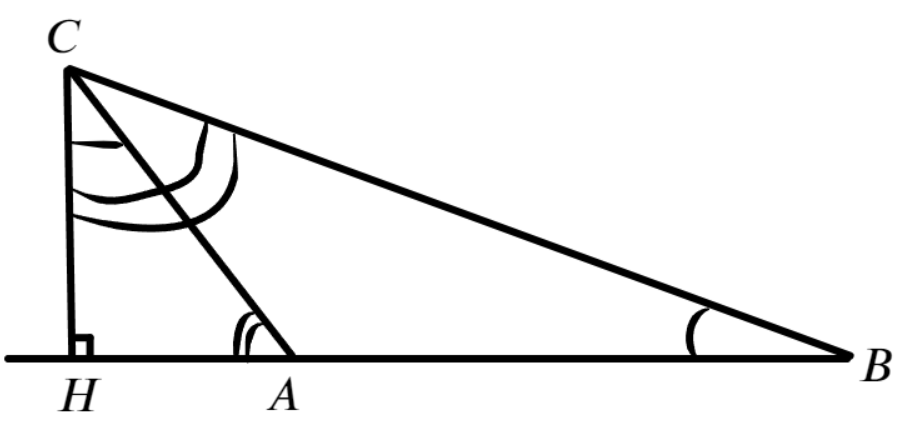
\includegraphics[scale=0.35]{g8-220.png}}
\end{figure}\\
Если взять $\angle A=110^\circ,\ \angle B=20^\circ,\ \angle C=50^\circ,$ то те же треугольники, что и в пункте а), будут подобны и соотношение также будет выполняться.\\
